\chapter{Experimental Evaluation}\label{\positionnumber} 
\section{Setup}\label{\positionnumber}
    \subsection*{Implementation}
        The implementation is written in C and currently has approximately $15 000$ lines of code.
        At the most basic level, it comprises data structures like hash tables, lists, queues, and Fibonacci heaps, but also record structures. 
        The latter are similar to the ones used in Neo4J. 
        The difference to the structures of Neo4J is that properties, labels, and relationship types are currently not supported.
        Besides that, the data structures are described as in Section~\ref{n4j}.
        The database only operates in-memory, implementing an access layer using the \mintinline{c}{expand} and \mintinline{c}{get_nodes} operations.
        Instead of using two files, two hash tables are used to store the records --- one for nodes and one for edges. \\
        The access layer atop, all traversal, shortest path algorithms, and the Louvain method is implemented. These algorithms are augmented to log the IDs of accessed nodes and relationships.
        Further, the static locality optimizing data layout algorithms of G-Store and ICBL are contained, along with the Louvain method and the incidence list's ordering.
        Additionally, routines for counting the number of accessed blocks based on the logged sequence of nodes and relationships and an importer for datasets from the SNAP dataset collection are implemented.
    
    
    \subsection*{Cost Model}
        The cost model used to quantify the locality improvement is based on the sequence of nodes and relationships that are accessed. 
        We assume that the cache or buffer has the size of exactly one block, such that only the accessed block is to be considered ``in memory''.
        First, the block number of the accessed record is calculated by 
        \[ \frac{\text{record ID} \cdot \text{record size}}{\text{block size}} \]
        As long as consecutive accesses to records produce the same block number, the access is counted as one block IO.
        Otherwise, --- i.e., if the block number changes --- it is counted as additional block IO. 
        If the block number change differs only by one block, it is counted as a sequential block IO.
        When considering the definition of block-based spatial locality
        \[ P(X_{t + \Delta} = B + \varepsilon | X_t = B) \]
        we set $\varepsilon$ to 8. 
        This would correspond to a system with a block size of $512$ Bytes and a page size of $4096$.
        Further, when also using prefetching, even larger values for $\varepsilon$ can occur.  \\
        The above-described model should correspond closely to how the disk is stored. 
        Besides an offset of one (or multiple) blocks for the maintenance of free blocks and eventually free slots, the block alignment is the same:
        All IDs in this schema are stored implicitly by the nodes' position in the file. 
        That is --- as described in Section~\ref{n4j}--- with a node size of 64 bytes when the node record starts at 192 bytes + header offset, then it has the ID $3$. \\
        Finally, we are only going to measure the number of block IOs and the number of non-sequential IOs as mentioned above and in Section~\ref{prob-def}.
    
    \subsection*{Data Sets and Queries}
        We use datasets from the Stanford Network Analysis Project~\autocite{snap}.
        More specifically we use datasets starting from $131$ nodes and $764$ edges, ranging to $1,134,890$ nodes and $2,987,624$ edges.
        All datasets that are used so far are unweighted, i.e. all edges have a weight of $1$.
        A summary of the considered networks is shown in Table~\ref{datasets}.
        \begin{table}
        \begin{center}
            \begin{tabular}[c]{l l r r p{5.8cm}} \toprule
                Name & Type & Nodes & Edges & Description \\ \midrule
                 C.elegans & Directed & $131$ & $764$ & Frontal part of the neural network of a C. elegans~\autocite{celegans} \\ [0.8cm]
                 Email & Directed & $1,005$ & $25,571$ & E-Mail traffic between european research institutions~\autocite{email} \\ [0.8cm]
                 DBLP & Undirected & $317,080$ & $1,049,866$ & Computer science citation network~\autocite{lj}. \\ [0.8cm]
                 Amazon & Undirected & $334,863$ & $925,872$ & Co-purchased items network crawled from Amazon~\autocite{lj}. \\ [0.8cm]
                 YouTube & Undirected & $1,134,890$ & $2,987,624$ & YouTube social network~\autocite{mislove}. \\ \bottomrule
            \end{tabular}
            \end{center}
            \caption{Details on the datasets that are used during evaluation.}
            \label{datasets}
        \end{table}
        The queries executed to gather the access sequences are breadth first searchm depth first search, Dijkstra's algorithm, the A$^*$ algorithm and the ALT algorithm. 
        The A$^*$ algorithm is supplied a perfect heuristic, that is, the Dijkstra algorithm's output starting from the target node. ALT is executed using five landmarks. \\
        As described above, the accessed nodes and relationship IDs are logged by the implementation of these algorithms.

    \subsection*{Environment}
        The evaluation is executed on a 2015 MacBook Pro with an Intel Core i5-4278U processor running at $2.6$ GHz, with a boost of $3.1$GHz. The bus width is 64 bits. 
        It was manufactured using a 22nm process, has two cores with two threads each, has $128$ KiB L1 with $64$ KiB for instructions and data each, $512$KiB L2 and 3MiB L3 Cache.
        The main memory consists of $2 \cdot 4$GiB SODIMM DDR3 RAM clocked at 1600 MHz by Micron Technology.
        We are not using the disk directly, but it may be indirectly used by the operating system when paging or swapping is exchanging pages, or process images.
        The disk is a $256$GB SSD produced by Samsung and uses the SATA protocol over the PCIe 3.0 x4 interface. A combination of 8 GiB RAM and a 10 GiB swap file was insufficient to support larger datasets for G-Store's and the ICBL record layout algorithms.
    
\section{Results}\label{\positionnumber}
    For each of the datasets, we applied five different layouts. 
    First, the layout was left as is, governed mainly by the input dataset's order.
    Second, we randomized the order.
    Third, the Louvain method is applied to partition the graph. The vertex records are then sorted based upon the partition stably. This means that if two records have the same partition number, the previous order is preserved.
    Fourth, the algorithm developed for G-Store is applied.
    Finally, ICBL orders the records.
     \begin{figure}[htp]
        \begin{center}
            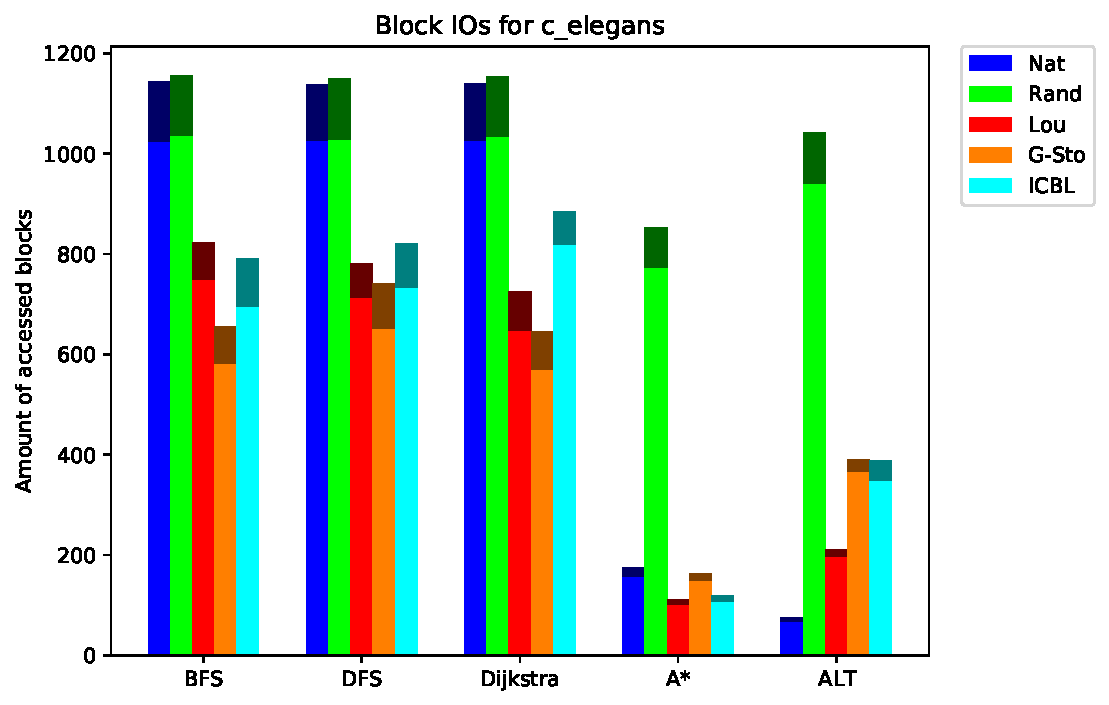
\includegraphics[keepaspectratio,width=0.7\textwidth]{img/07-eval/c_elegans_Block_unsorted_io_comparison.pdf}
        \end{center}
        \caption{Comparison of the number of block accesses using the layouts produced by mentioned methods when executing the algorithms.} 
        \label{celegans_b}
    \end{figure}
    
    The IDs of the vertex records were reassigned correspondingly and mapped to blocks using the above orders. 
    Relationships were then remapped, matching the vertex order based on outgoing connections.\\
    Consider the results shown in Figure~\ref{celegans_b}. In this figure, we used the C. elegans dataset.
    We can see that the natural and the random layout imply additional block IOs by a factor of approximately 1.5 for traversal-based algorithms that visit all nodes.
    For the algorithms that traverse only a fraction of the nodes, the results are not so precise. For A$^*$, the partition-based layouts are all slightly better, while for ALT, they are worse up to a factor of approximately 6.
    
    \begin{figure}[htp]
        \begin{center}
            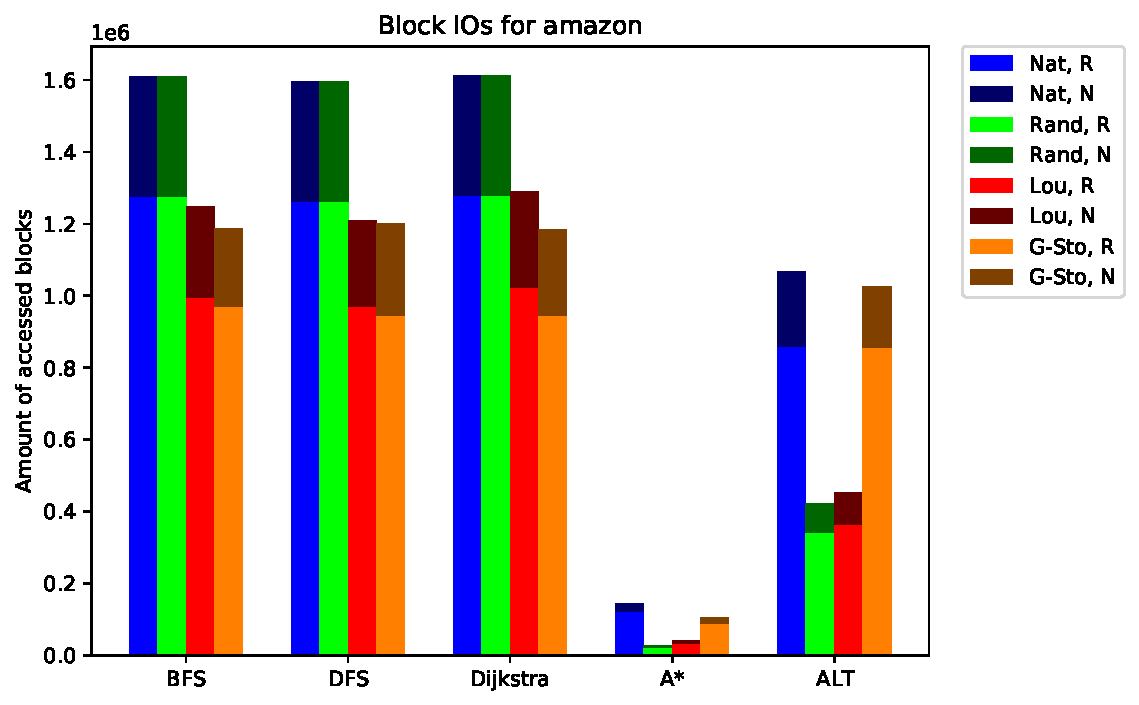
\includegraphics[keepaspectratio,width=0.7\textwidth]{img/07-eval/amazon_Block_unsorted_io_comparison.pdf}
        \end{center}
        \caption{Comparison of the number of block accesses using the layouts produced by mentioned methods when executing the algorithms on the Amazon dataset.} 
        \label{am-b}
    \end{figure}
    \begin{figure}[htp]
        \begin{center}
            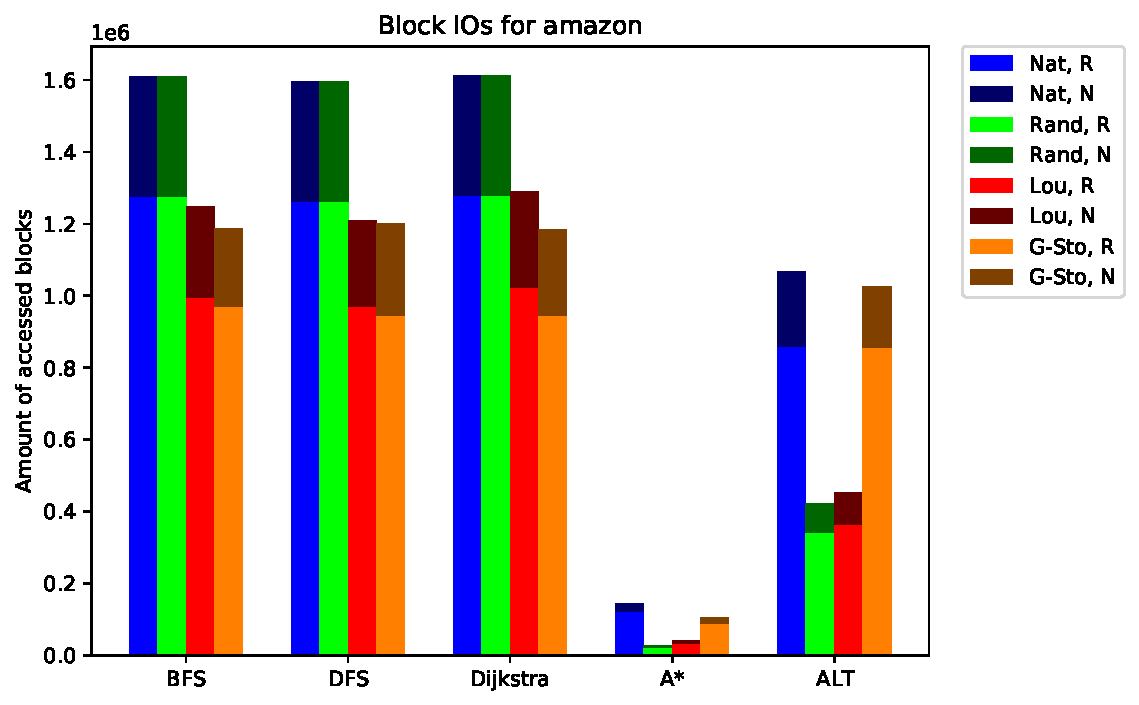
\includegraphics[keepaspectratio,width=0.7\textwidth]{img/07-eval/amazon_Block_unsorted_io_comparison.pdf}
        \end{center}
        \caption{Comparison of the number of block accesses using the layouts produced by mentioned methods when executing the algorithms on the Amazon dataset.} 
        \label{am-p}
    \end{figure}
    
    We have seen how the results look on the smallest dataset. Now let us consider the largest dataset that was used.
    In Figure~\ref{yt-b}, ICBL is not shown.
    ICBL relies on an adapted version of K-Means clustering, where the centers are chosen by the maximum of the aggregated diffusions set of the cluster. 
    This leads to the behavior that hub vertices are the ones that are chosen most often.
In this situation, the following assignment of the vertices assigns most of the nodes to one cluster. When the initial centers are peripheral, a few clusters get vast, and many are relatively small. In the worst-case, most of the nodes end up in one cluster. The worst-case happened quite often in praxis. The next step is hierarchical clustering, with the distance function being the minimal distance between nodes in the respective subcluster. In other words, one either recomputes the distance for each merge for all vertices in both clusters pairwise, or one stores the pairwise distance matrix.
    This matrix has the size $|V|^2 \cdot 4$. For $300000$, this would result in an allocation of 335 GiB, which is unfeasible on most machines.
    The authors of this method did not describe how to deal with this scenario or make sure the clusters stay balanced in size during coarse clustering. It is thus excluded from datasets that would result in allocation errors.
    
    \begin{figure}[htp]
        \begin{center}
            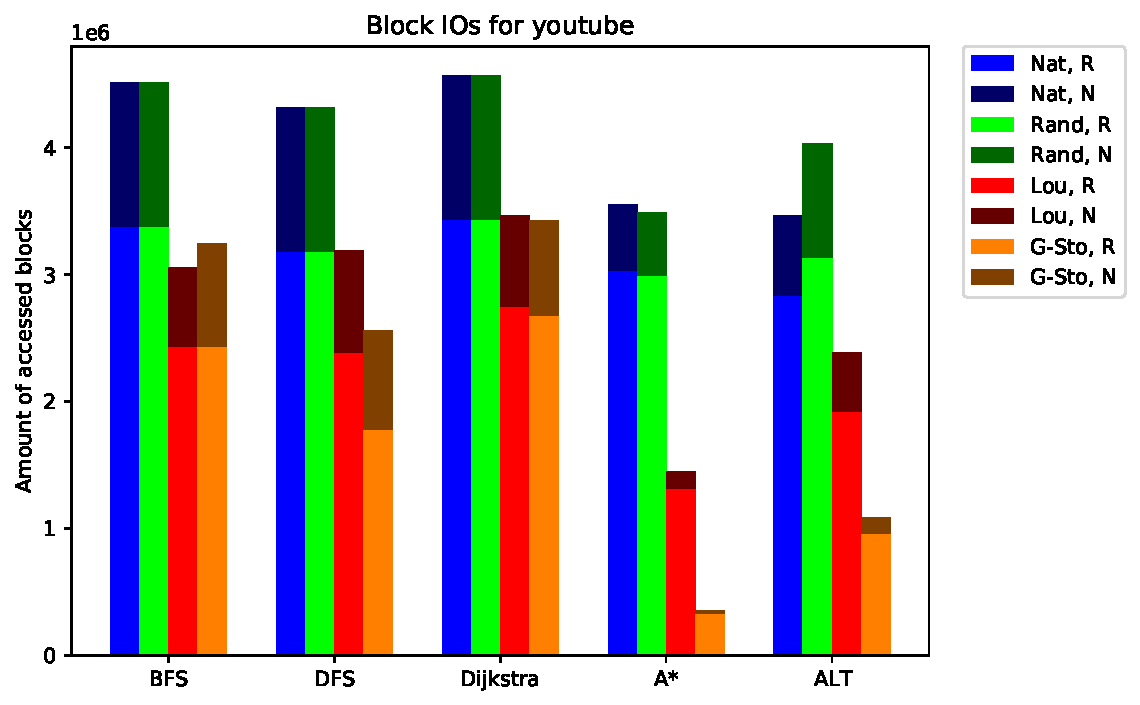
\includegraphics[keepaspectratio,width=0.7\textwidth]{img/07-eval/youtube_Block_unsorted_io_comparison.pdf}
        \end{center}
        \caption{Comparison of the number of block accesses using the layouts produced by mentioned methods when executing the algorithms on the YouTube dataset.}
        \label{yt-b}
    \end{figure}
    
    
    As the datasets grow in size, the partition-based layouts tend to outperform the random and natural layout on all queries, as shown in Figure~\ref{yt-b}, which visualized the amount of block IOs on the YouTube dataset.    
    % Point 1 Youtube both

    \begin{figure}[htp]
        \begin{center}
            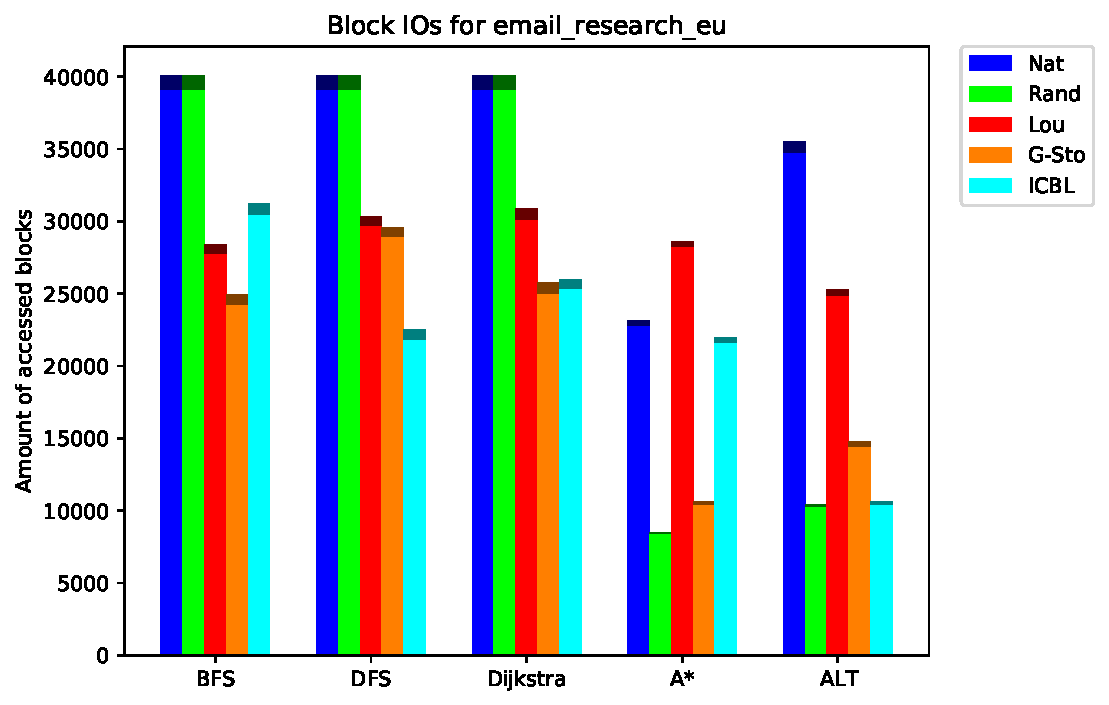
\includegraphics[keepaspectratio,width=0.7\textwidth]{img/07-eval/email_research_eu_Block_unsorted_io_comparison.pdf}
        \end{center}
        \caption{Comparison of the number of block accesses using the layouts produced by mentioned methods when executing the algorithms on the Email dataset.} 
        \label{email-block}
    \end{figure}
    
    Regarding spatial locality, Figure~\ref{am-b} shows the block-based IOs for the amazon dataset. Figure~\ref{am-p} shows the page-based IOs for the same dataset. When access is block-based, G-Store performs approximately equivalent to the natural layout, while on page-based access, it uses only half of the accesses. During no experiment, the total theoretical gain of 8 was achieved between block- and page-oriented IO. \\
    
    The Louvain method performs overall also better than the natural and random layouts. However, it performs most times worse than G-Store's layout method, as it has no means to order partitions. Also, it is in contrast to the other methods per se non-hierarchical concerning specific block size and its output. In Figure~\ref{email-block} we can see that it performs by far worst in comparison with the other partition-based methods. When applying the A$^*$ algorithm is even worse than the natural layout.
    
      \begin{figure}[htp]
        \begin{center}
            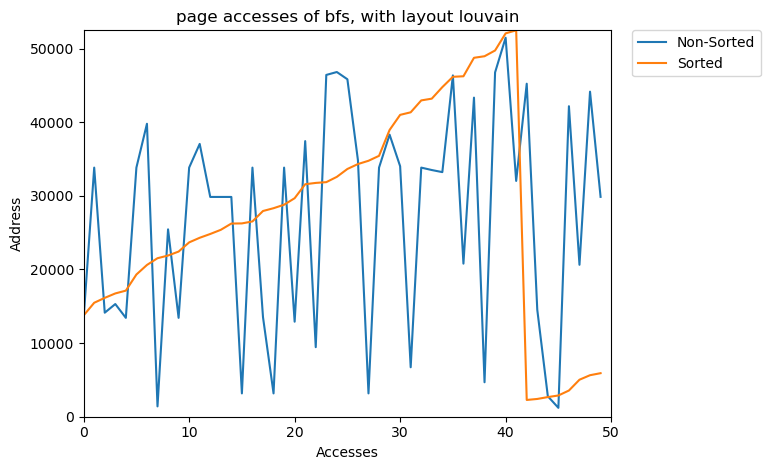
\includegraphics[keepaspectratio,width=0.5\textwidth]{img/07-eval/youtube_louvain_bfs_page_sil_access_seq.png}
        \end{center}
        \caption{A sequence of 50 page access with sorted incidence list when traversing the YouTube social network graph laid out using the Louvain method breadth first} 
        \label{yt-sq}
    \end{figure}
    
    
    % Point 2 sequences
    Finally, sorting the incidence lists has an impact on the sequence in which blocks are accessed. 
    In the following figures, 50 consecutive accesses are visualized. These are taken randomly from all accesses (visualizing more or even all accesses leads to a fully colored square). However, the accesses are not synchronized in the sense that they are answering the same request. They only show access $x$ to access $x + 50$. Using sorted incidence lists leads to fewer accesses (see, for example, Table~\ref{yt-s} and Table~\ref{yt-uns}).
    Figure~\ref{yt-sq} shows how many of the $50$ pages across a range of approximately $35000$ are accessed in a perfect monotone increasing sub-sequence. This access sequence is generated using the YouTube dataset, the BFS traversal algorithm, and the Louvain method-based record layout. Accesses without a sorted incidence list are shown in blue.

    Similar sequentially accesses are shown in Figure~\ref{dblp_good} for the DBLP dataset laid out using G-Store's method and the ALT algorithm as query. This time it spans approximately $130000$ blocks and needs 3 monotone increasing subsequences.
    \begin{figure}[htp]
        \begin{center}
            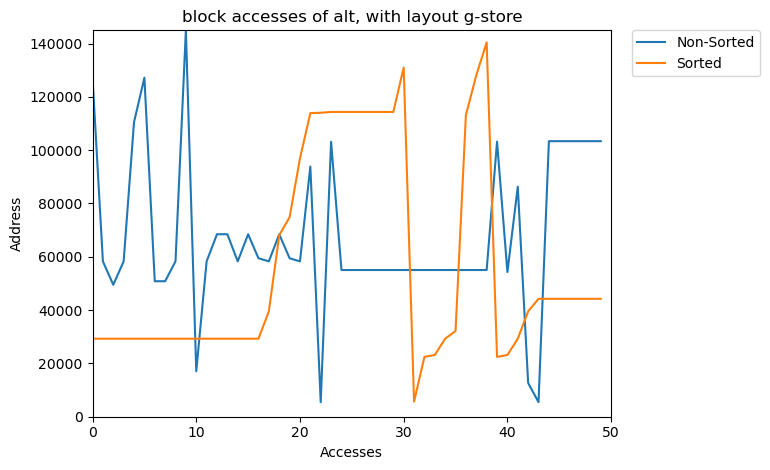
\includegraphics[keepaspectratio,width=0.5\textwidth]{img/07-eval/dblp_g-store_alt_block_sil_access_seq.png}
        \end{center}
        \caption{A sequence of 50 page access with sorted incidence list when executing the ALT algorithm on the DBLP citation network graph laid out using G-Store's method.} 
        \label{dblp_good}
    \end{figure}
    
    However this is not always the case. In Figure~\ref{dblp_ng} we can see that with both sorted and unsorted incidence lists, the accesses jump quite a lot when the natural layout is preserved.
    \begin{figure}[htp]
        \begin{center}
            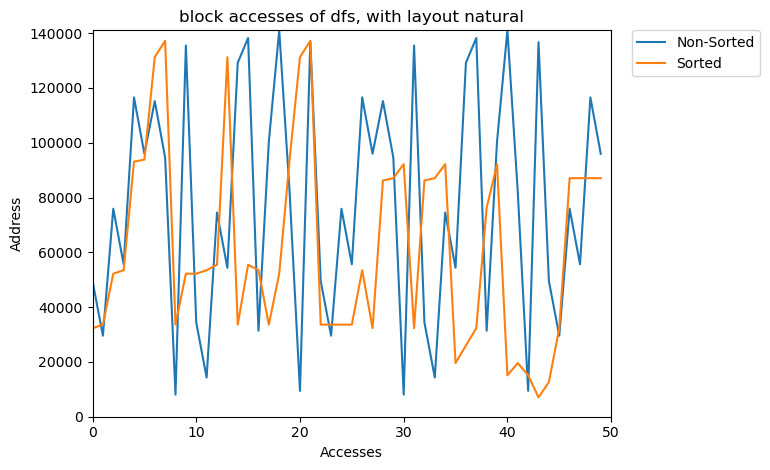
\includegraphics[keepaspectratio,width=0.5\textwidth]{img/07-eval/dblp_natural_dfs_block_sil_access_seq.png}
        \end{center}
        \caption{A sequence of 50 page access with sorted incidence list when executing a depth-first traversal on the DBLP citation network graph with preserved natural layout.} 
        \label{dblp_ng}
    \end{figure}
    
     The key points that the results above show can be summarized as follows.
    \begin{itemize}
     \item Static rearrangement methods indeed decrease the overall number of block accesses and thus increase the temporal locality of all blocks and spatial for pages.
     \item Sorting the incidence lists leads to often sequential access sequences.
     \item ICBL's coarse clustering is crucial for larger datasets but is probably not described fully in the papers.
     If it fails to balance the size of the cluster, systems will run out of memory.
     \item The Louvain method sometimes performs well, sometimes not. This qualitative degradation is due to not ordering the blocks within a partition and the non-hierarchical approach.
    \end{itemize}
